\documentclass[10pt,twocolumn]{article}
\usepackage[a4paper,top=2.2cm,bottom=2.4cm,left=1.8cm,right=1.8cm,columnsep=0.7cm]{geometry}
\usepackage{xcolor}
\usepackage{graphicx}
\usepackage{booktabs}
\usepackage{amsmath,amssymb}
\usepackage{microtype}
\usepackage[numbers,sort&compress]{natbib}
\usepackage[colorlinks=true,linkcolor=blue,citecolor=blue,urlcolor=blue]{hyperref}
\usepackage{times}
\usepackage{caption}
\captionsetup{font=small,labelfont=bf}

\setlength{\parskip}{0pt}
\newcommand{\meteor}{METEOR}
\newcommand{\eg}{e.g.,}
\newcommand{\ie}{i.e.,}

\title{\textbf{\meteor{}: From Raw Surround-View Recordings to a Seven-Task\\
Driving Network without Human Labels or Human-Written Code}}
\author{Dan Umeda\\
TIER IV, Inc.\\
\texttt{https://github.com/tier4/METEOR}}
\date{}

\begin{document}
\maketitle

\begin{abstract}
We present \meteor{} (Multi-task Estimation of Traffic Elements, Objects and
Roads), a surround-view, camera-only network that predicts seven driving tasks
in a single forward pass---BEV lane segmentation, metric depth, oriented 3D
boxes, 21-class 2D segmentation, 10-class 2D detection, 3D semantic occupancy,
and an end-to-end driving output (trajectory, steering, acceleration,
braking)---and, equally importantly, the fully automated pipeline that builds
it. Every supervision signal is distilled offline from raw eight-camera
recordings of the Co-MLOps Data Recording System by an autolabel factory
built on the CoMET autolabeling foundation, which combines LiDAR, ego-motion
and 2D panoptic pseudo-labels; no human annotated a single box, mask, or
trajectory. The network couples a shared image backbone with a
\emph{depth-gated inverse perspective mapping} that uses predicted depth as a
visibility gate for geometric BEV projection, and restricts itself to
TensorRT-exportable operators (38.3\,M parameters, 3.1\,TFLOPs for eight
cameras). We describe a rolling-round training methodology in which data
conversion, ground-truth refinement and multi-task training run concurrently,
and report a series of measurement-driven loss corrections---curvature-weighted
imitation, coverage-preserving thin-class rasterisation, and small-object
retention---each of which repaired a quantified failure mode. On a held-out
recording, \meteor{} reaches 0.292 BEV lane mIoU, 1.60\,m depth MAE, and a
3\,s trajectory ADE of 0.76\,m (0.72\,m on curves, brought down from 2.31\,m
by curvature weighting). Finally, the entire system---models, pipeline,
training and analysis code, and this manuscript---was authored by a large
language model agent (Claude Fable~5) operating autonomously under human
direction, which we discuss as a development methodology.
\end{abstract}

\section{Introduction}
Perception stacks for automated driving are conventionally built one task at a
time, each with its own annotation campaign. Labeling is the dominant cost:
boxes, masks, lane geometry, and occupancy grids each require dedicated
tooling and thousands of hours of human effort, and every new task restarts
the cycle. At the same time, modern data-collection platforms record far more
information than any annotation budget can absorb---synchronized surround
cameras, LiDAR, and centimeter-level ego-motion---which in principle contain
almost everything the labels would say.

This paper describes an attempt to close that loop completely. Starting from
raw recordings of the Co-MLOps Data Recording System
(DRS)\footnote{\url{https://co-mlops.tier4.jp/}}---eight synchronized cameras,
a concatenated LiDAR, ego-poses, and machine-generated 2D panoptic
labels---we build \emph{seven} supervision signals and train a single
multi-task network, with two hard constraints that we believe make the result
practically interesting:

\begin{itemize}\itemsep1pt
\item \textbf{Zero human labels.} All ground truth is produced by an
autolabel factory built on CoMET, the autolabeling foundation of the Co-MLOps
project. Humans never annotate; they only record.
\item \textbf{Zero human-written code.} The complete system---ground-truth
extractors, model, trainer, demo tooling, documentation, and this
paper---was written by an LLM agent (Claude Fable~5) working autonomously
under human direction (Sec.~\ref{sec:agent}).
\end{itemize}

\noindent Our contributions are:
\begin{enumerate}\itemsep1pt
\item \textbf{An autolabel factory for seven tasks} (Sec.~\ref{sec:factory}):
a ten-stage, per-scene, resumable pipeline that turns raw DRS recordings into
BEV lane maps, dense metric depth, camera-confirmed oriented 3D boxes,
21-class 2D segmentation, 10-class 2D boxes, end-to-end driving targets
derived purely from ego-motion, and 3D semantic occupancy with ray-carved free
space---plus the quality gates that make such labels trainable.
\item \textbf{\meteor{}} (Sec.~\ref{sec:arch}): a 38.3\,M-parameter,
3.1\,TFLOP surround-view network whose depth-gated IPM converts image features
to BEV using only TensorRT-friendly operators, and whose head design follows
an explicit capacity rule---\emph{parameters at low resolution, compute at
high resolution}---that adds tasks at $<5\%$ marginal cost.
\item \textbf{A rolling-round training methodology}
(Sec.~\ref{sec:training}): data conversion, GT re-extraction and training run
concurrently; each $\sim$24\,h round folds in newly converted scenes and
measurement-driven loss fixes. We document three such fixes (curvature
weighting for imitation, coverage-based thin-class rasterisation, small-object
retention) with the quantified failures that motivated them.
\item \textbf{An agent-authored system} (Sec.~\ref{sec:agent}): to our
knowledge the first published driving-perception system in which not only the
labels but all engineering artefacts were machine-generated, with humans
reduced to specification and review.
\end{enumerate}

\section{Related Work}
\textbf{Camera-to-BEV perception.} Lifting multi-camera features to BEV is
commonly done by depth-distribution splatting (LSS~\citep{philion2020lss},
BEVDepth~\citep{li2023bevdepth}) or by attention
(BEVFormer~\citep{li2022bevformer}, TPVFormer~\citep{huang2023tpvformer}).
\meteor{} instead uses a \emph{pull-based} formulation: BEV grid points are
projected into the cameras and sample features weighted by the predicted
depth probability at their geometric range. This inverts LSS-style splatting
(gather instead of scatter) and avoids attention entirely, which keeps the
graph exportable to TensorRT without plugins.

\textbf{Multi-task and end-to-end driving.} UniAD~\citep{hu2023uniad} showed
that planning benefits from jointly trained perception; MapTR~\citep{liao2023maptr}
popularised vectorised lane learning; CenterPoint~\citep{yin2021centerpoint}
and CenterNet~\citep{zhou2019objects} anchor our detection heads;
Occ3D~\citep{tian2023occ3d} defines the occupancy task we target. Conditional
imitation~\citep{codevilla2018cil} underlies our E2E head, conditioned on
current speed. \meteor{} differs in breadth (seven tasks in one pass) and in
its supervision source (no human labels at any stage).

\textbf{Auto-labeling.} Offboard auto-labeling with strong LiDAR detectors is
well established~\citep{qi2021offboard}. Our factory differs in that it needs
no trained detector for most tasks: lanes, depth, occupancy, and E2E targets
come from geometry (LiDAR accumulation, ego-motion, ray casting) fused with
2D panoptic pseudo-labels, and 3D boxes are only \emph{filtered}, not
generated, by learned components.

\section{The Autolabel Factory}
\label{sec:factory}
The factory consumes t4dataset-format recordings (a nuScenes-like
schema~\citep{caesar2020nuscenes}: keyframed samples, calibrated sensors,
ego-poses, LiDAR sweeps, and 2D panoptic annotations stored as COCO
run-length masks). A single driver executes ten stages per scene; every stage
skips existing outputs, so the factory is resumable and runs scene-parallel
alongside training. We summarise each supervision signal; exact recipes are in
the repository documentation.

\subsection{BEV lane ground truth}
LiDAR points from every keyframe are projected into all cameras (pinhole and
equidistant fisheye) and take road-surface classes from the panoptic masks;
thin classes (lane line, stop line, road edge, marking) are only accepted
within 15\,m, where the pixel-to-ground error is sub-cell. Ego-poses
accumulate the labeled points into a global 0.1\,m grid over the whole scene,
which is rasterised with hit-count priorities and a 20\,m observation-distance
mask. The raster is then \emph{vectorised}---skeletonisation, spur pruning,
Douglas-Peucker simplification, and dash-gap linking---and per-frame GT crops
($\pm$80$\times$$\pm$50\,m at 0.2\,m) are re-rendered hybrid-style: area
classes from the raster, line classes re-drawn from the vectors at fixed
width. Two guards proved essential: enclosed road holes ($\le$400 cells,
LiDAR shadows) are filled, and opposing carriageways are removed by an
ego-connected-component filter with a 30\% revert guard that protects wide
intersections from being wiped.

\subsection{Dense metric depth}
Per camera, LiDAR points splat a sparse min-depth image at stride 4. Depth is
densified by linear interpolation \emph{over the union of road and
road-paint panoptic segments}---interpolating paint separately leaves holes
around every lane line---followed by a geometric ground-plane fill restricted
to rays within 50$^\circ$ of downward (a guard against fisheye-calibration
tails), a same-segment nearest fill, and per-segment medians. Sky and ego
pixels receive fixed codes. The result is a 64-bin (1.25\,m) target at
108$\times$192 for all eight cameras.

\subsection{Camera-confirmed 3D boxes}
The recordings carry LiDAR-frame 3D annotations whose instance IDs are
disjoint from the 2D panoptic instances, so association must be geometric: a
3D box is kept only if its eight projected corners overlap a same-class 2D
annotation in some camera (intersection over minimum area $>0.3$). This
removes fully occluded objects that a camera-only network cannot see,
which otherwise poison the BEV detection loss.

\subsection{2D segmentation and 2D boxes}
Both taxonomies are CSV-driven so that class definitions are data, not code:
21 semantic classes and 10 instance classes with Cityscapes-like colours. Two
findings matter. (i)~\emph{Thin classes do not survive naive downsampling}: at
stride-4 GT resolution a lane line is $\sim$0.3\,px wide and nearest-neighbour
resizing deletes it; rasterising a cell as the thin class when $>12\%$ of its
footprint is covered recovered $+49\%$ lane pixels and turned broken dashes
into connected supervision. (ii)~\emph{Silent truncation deletes exactly the
rare classes}: with a per-camera box budget of 32, area-sorted retention
dropped 29\% of annotations in crowded scenes---all of them small (cones,
traffic lights, distant unknowns). Raising the budget to 96 and adding
per-class positive weights fixed the small-object classes.

\subsection{End-to-end driving targets from ego-motion}
No CAN bus data is available, so all driving targets derive from ego-poses:
future positions at $+0.5\ldots+3.0$\,s transformed into the current ego frame
(six waypoints); speed and acceleration by smoothed finite differences;
steering via a bicycle model $\delta=\arctan(L\dot\psi/v)$ with wheelbase
$L{=}2.8$\,m, masked below 0.5\,m/s; braking as acceleration below
$-0.5$\,m/s$^2$. Instantaneous signals are written for \emph{every} frame---an
early version left the speed field zero when the 3\,s future was missing at
scene tails, and the deployed model, conditioned on that bogus zero, predicted
``hold'' at 80\,km/h. Trajectory targets carry a validity mask instead.

\subsection{3D semantic occupancy}
Ego-frame voxels ($16{\times}200{\times}200$ at 0.4\,m; $\pm$40\,m,
$z\in[-1,5.4)$\,m) with ten classes plus \emph{unknown}. Points from $\pm$8
strided frames are labeled by sampling the cached 21-class segmentation GT
(a factor-15 speedup over re-decoding panoptic masks) and accumulated via
ego-poses; \emph{dynamic} classes (vehicles, two-wheelers, pedestrians) are
taken from $\pm$1 frames only, since full accumulation smears moving objects
into lane-long streaks. Free space is carved by ray-stepping the current
sweep at 0.4\,m intervals; coarser stepping (an early 1.7\,m version) left
most above-road voxels unknown, and the trained model hallucinated confident
structure in exactly those unsupervised regions.

\subsection{Quality gates}
Three train-time filters removed systematic label noise: scene-end trimming
(the last 10 frames lack forward accumulation), a per-frame GT-coverage
filter (labeled fraction $\ge$3\% in the $\pm$30\,m band and $\ge$0.5\% in
the 30--80\,m band; long-stationary frames fail this), and indoor/underground
scene rejection via panoptic sky statistics, because NDT pose drift makes
kinematic filters unreliable there.

\begin{figure*}[t]
\centering

\includegraphics[width=0.98\textwidth]{figs/architecture.png}
\caption{\textbf{\meteor{} architecture.} A shared ResNet-34+FPN yields a
stride-4 feature per camera, consumed by four image-space heads. The
parameter-free depth-gated IPM projects BEV grid points into the cameras and
gathers context features weighted by the predicted depth probability at each
point's range; four BEV-space heads (lanes, 3D boxes, occupancy, E2E) share
the resulting 96-channel BEV feature. Green lines denote task outputs; all
operators are TensorRT-exportable.}
\label{fig:arch}
\end{figure*}

\section{\meteor{} Architecture}
\label{sec:arch}
Fig.~\ref{fig:arch} shows the network. Eight 768$\times$432 images pass
through a shared ResNet-34~\citep{he2016resnet} with an FPN~\citep{lin2017fpn}
that fuses all levels at stride 4 into a 160-channel feature $f$.

\subsection{Depth-gated IPM}
A fixed BEV grid ($800{\times}500$ at 0.2\,m; $\pm$80$\times$$\pm$50\,m,
$z{=}0$) is projected into every camera by the calibrated $K,T$. At each
projection we \texttt{grid\_sample} a 96-channel context feature $c$ and the
predicted depth distribution $p(d)$, then \texttt{gather} the probability at
the point's geometric range $r$:
\begin{equation}
w_{i,n} = p_n\!\left(d{=}r_{i,n}\right) + \epsilon,\qquad
b_i = \frac{\sum_n w_{i,n}\, c_n(u_{i,n})}{\sum_n w_{i,n}},
\end{equation}
where $n$ indexes cameras, $i$ BEV cells, and $\epsilon{=}0.05$ keeps the
gate leaky. Depth thus acts as a \emph{visibility valve}: features flow into a
BEV cell only from cameras whose predicted depth agrees with that cell's
range, suppressing the occlusion bleed-through that plagues plain IPM. The
block has no parameters and uses only \texttt{grid\_sample}/\texttt{gather},
in contrast to scatter-based splatting~\citep{philion2020lss} or
attention~\citep{li2022bevformer}.

\subsection{Heads and capacity allocation}
Table~\ref{tab:cost} lists all stages. Two rules organise the design:

\textbf{Parameters at low resolution, compute at high resolution.} Early
heads ran 3$\times$3 convolutions at stride 4---the worst corner of the
FLOPs/params trade-off. The redesigned 2D heads push channels into
stride-8/16 towers (encoder--decoder for segmentation; a three-scale
CenterNet pyramid for detection, with GT assigned by box size) and touch
stride 4 only through 1$\times$1 laterals: an 18$\times$ parameter increase
for $\sim$2$\times$ FLOPs, worth $+0.076$ 2D-seg mIoU
(Sec.~\ref{sec:exp:capacity}).

\textbf{Tasks are cheap on a shared BEV.} The occupancy head (a stride-2 stem
on a $\pm$40\,m crop predicting $10{\times}16$ channels) and the E2E head (a
strided pyramid pooled to 256-d, concatenated with speed $v_0$, and decoded by
an MLP) together cost 3\% of total compute.

\begin{table}[t]
\centering\small
\caption{Measured cost per stage (eight cameras, 768$\times$432).}
\label{tab:cost}
\begin{tabular}{@{}lrrr@{}}
\toprule
Stage & Params & GFLOPs & Share\\
\midrule
Backbone + FPN & 21.66\,M & 475 & 15\%\\
Depth decoder & 3.29\,M & 1093 & 35\%\\
BEV lane decoder & 1.16\,M & 933 & 30\%\\
2D segmentation head & 4.18\,M & 219 & 7\%\\
2D detection head & 2.85\,M & 219 & 7\%\\
3D box head & 0.41\,M & 82 & 3\%\\
Occupancy head & 0.70\,M & 55 & 2\%\\
E2E head & 4.04\,M & 37 & 1\%\\
Context + IPM & 0.02\,M & 6 & $<$1\%\\
\midrule
Total & 38.31\,M & $\sim$3118 & \\
\bottomrule
\end{tabular}
\end{table}

\section{Training}
\label{sec:training}

\subsection{Multi-task loss}
The total loss is a weighted sum over tasks: BEV lanes (class-weighted
cross-entropy with trained background, Lov\'asz-softmax~\citep{berman2018lovasz},
boundary re-weighting, Tversky~\citep{salehi2017tversky} on line classes, Dice
on crosswalks, and far-row weighting), depth (label-smoothed bin
cross-entropy plus an L1 penalty on expected metric depth), 3D boxes
(Gaussian focal~\citep{lin2017focal,zhou2019objects} + centre L1), 2D
segmentation and detection (class- and camera-weighted variants), occupancy
(class-weighted cross-entropy ignoring unknown voxels), and E2E (below). Aux
losses return a graph-preserving zero on all-ignore batches---during rolling
GT re-extraction whole batches can be unlabeled, and an unguarded mean
cross-entropy returns NaN and destroys training within 50 steps.

\subsection{Measurement-driven loss corrections}
\label{sec:fixes}
Three corrections were made \emph{after} quantifying a failure, and we report
them as results in Sec.~\ref{sec:exp}: (i)~\textbf{curvature weighting}: 83\%
of frames are near-straight and longitudinal waypoint magnitudes exceed
lateral ones 18$\times$, so plain L1 learns a go-straight prior; we weight
lateral errors 4$\times$ and scale each sample by $1+\min(|y_{3s}|,6)/1.5$.
(ii)~\textbf{coverage-based thin-class rasterisation} and
(iii)~\textbf{small-object retention} as described in Sec.~3.4, paired with
per-class positive weights in both detection heads and a near-range
($<$20\,m) positive boost for vulnerable road users in the 3D head.

\subsection{Rolling rounds}
Training proceeds in $\sim$24\,h rounds on seven GPUs. Each round refreshes
the scene list with newly converted recordings, warm-starts from the previous
best checkpoint (shape-mismatched heads are dropped and re-initialised, so
class-count changes retrain only the affected head), and applies whatever GT
or loss fixes the previous round's metrics motivated. Nine rounds and four new
task heads shipped in the project's first three days; the same loop is
designed to run for months as the factory converts the full corpus.

\section{Experiments}
\label{sec:exp}

\subsection{Setup}
Data: $\sim$2{,}000 scenes from two vehicle platforms (1{,}120 from an
initial corpus; a second 5{,}282-scene corpus is converted progressively and
folded in round by round). Validation is one held-out recording session (273
scenes) never used for training. Training: 7$\times$ data-parallel, batch 2
per GPU, AdamW, cosine schedule, $10^{-4}$ peak LR, 46k samples per epoch.
All numbers below are single-model, single-pass; no test-time augmentation.

\subsection{Main results}
\begin{table}[t]
\centering\small
\caption{Validation results on a held-out recording.}
\label{tab:main}
\begin{tabular}{@{}lr@{}}
\toprule
Metric & Value\\
\midrule
BEV lane mIoU (8 classes + bg) & 0.292\\
2D segmentation mIoU (21 classes) & 0.451\\
\quad lane line / pole IoU & 0.483 / 0.449\\
Depth MAE (0--80\,m, 8 cams) & 1.60\,m\\
E2E trajectory ADE / FDE (3\,s) & 0.76\,m / 1.65\,m\\
E2E curve ADE ($|y_{3s}|>2$\,m) & 0.72\,m\\
Steering MAE / brake accuracy & 0.027\,rad / 0.81\\
Occupancy road IoU (0--10 / 10--20 / 20--40\,m) & 0.63 / 0.64 / 0.64\\
\bottomrule
\end{tabular}
\end{table}

Table~\ref{tab:main} summarises the current operating point. We stress the
context: every number is achieved \emph{without a single human label}, and
the validation recording is from a different day and route than all training
data. Fig.~\ref{fig:qual} shows qualitative output.

\subsection{Curvature weighting for imitation}
\label{sec:exp:curve}
Binning validation frames by ground-truth lateral displacement at 3\,s
exposed the go-straight prior of the unweighted model: ADE was 0.62\,m on
straight frames but 1.30\,m at 2--4\,m lateral and \textbf{2.29\,m} beyond
4\,m---3.7$\times$ worse than straight, hidden by an aggregate ADE of
0.86\,m because 76\% of validation frames are straight. One round of
curvature-weighted training (Sec.~\ref{sec:fixes}) brought the curve subset to
\textbf{1.07\,m} and a second to \textbf{0.72\,m}, at no cost to straight
frames (aggregate ADE improved to 0.76\,m). We consider the diagnosis-metric
(curve-conditioned ADE, reported every epoch) as important as the fix: without
it the regression would have been invisible.

\subsection{Head capacity re-balancing}
\label{sec:exp:capacity}
Replacing the stride-4 2D heads with the low-resolution-parameter design
(Sec.~\ref{sec:arch}) and fixing small-object GT retention raised 2D-seg mIoU
from 0.375 to \textbf{0.451} in one round (lane 0.402$\to$0.483, pole
0.244$\to$0.449) and enabled detection of classes that had never fired before
(traffic lights, distant signs, road obstacles), at $+10\%$ total FLOPs and
$+37\%$ parameters.

\subsection{Occupancy supervision density}
With 1.7\,m ray steps, most above-road voxels remained \emph{unknown} and the
model hallucinated high-confidence structure there (a solid ``slab'' over the
road in 3D renderings), while measured road IoU was unaffected---the errors
live exactly where no supervision exists. Densifying carving to one sample
per 0.4\,m voxel multiplies free-space supervision and is expected to remove
the hallucination; per-range road IoU (Table~\ref{tab:main}) already shows no
near-field deficit, countering the visual impression given by top-down
renderings that flatten hallucinated upper voxels onto the road.

\begin{figure}[t]
\centering
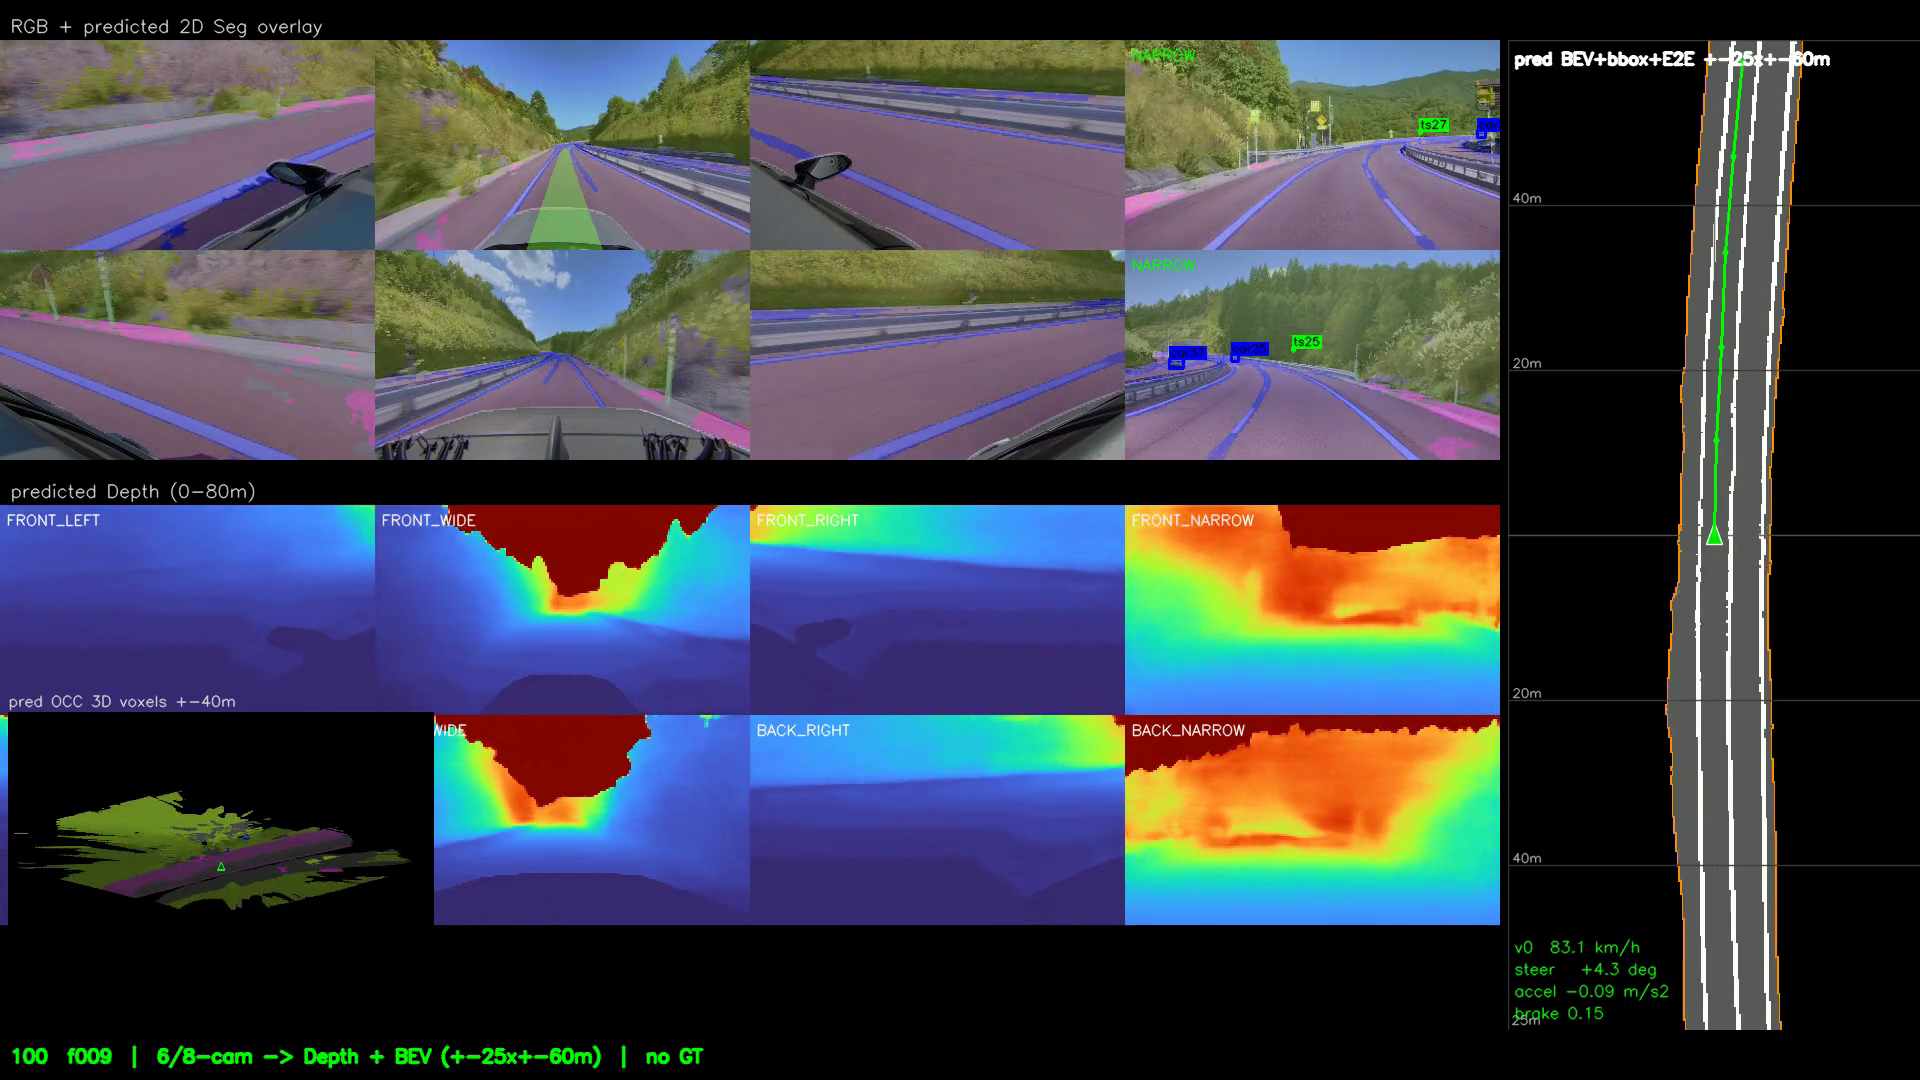
\includegraphics[width=0.99\linewidth]{figs/qual_inference.png}\\[2pt]
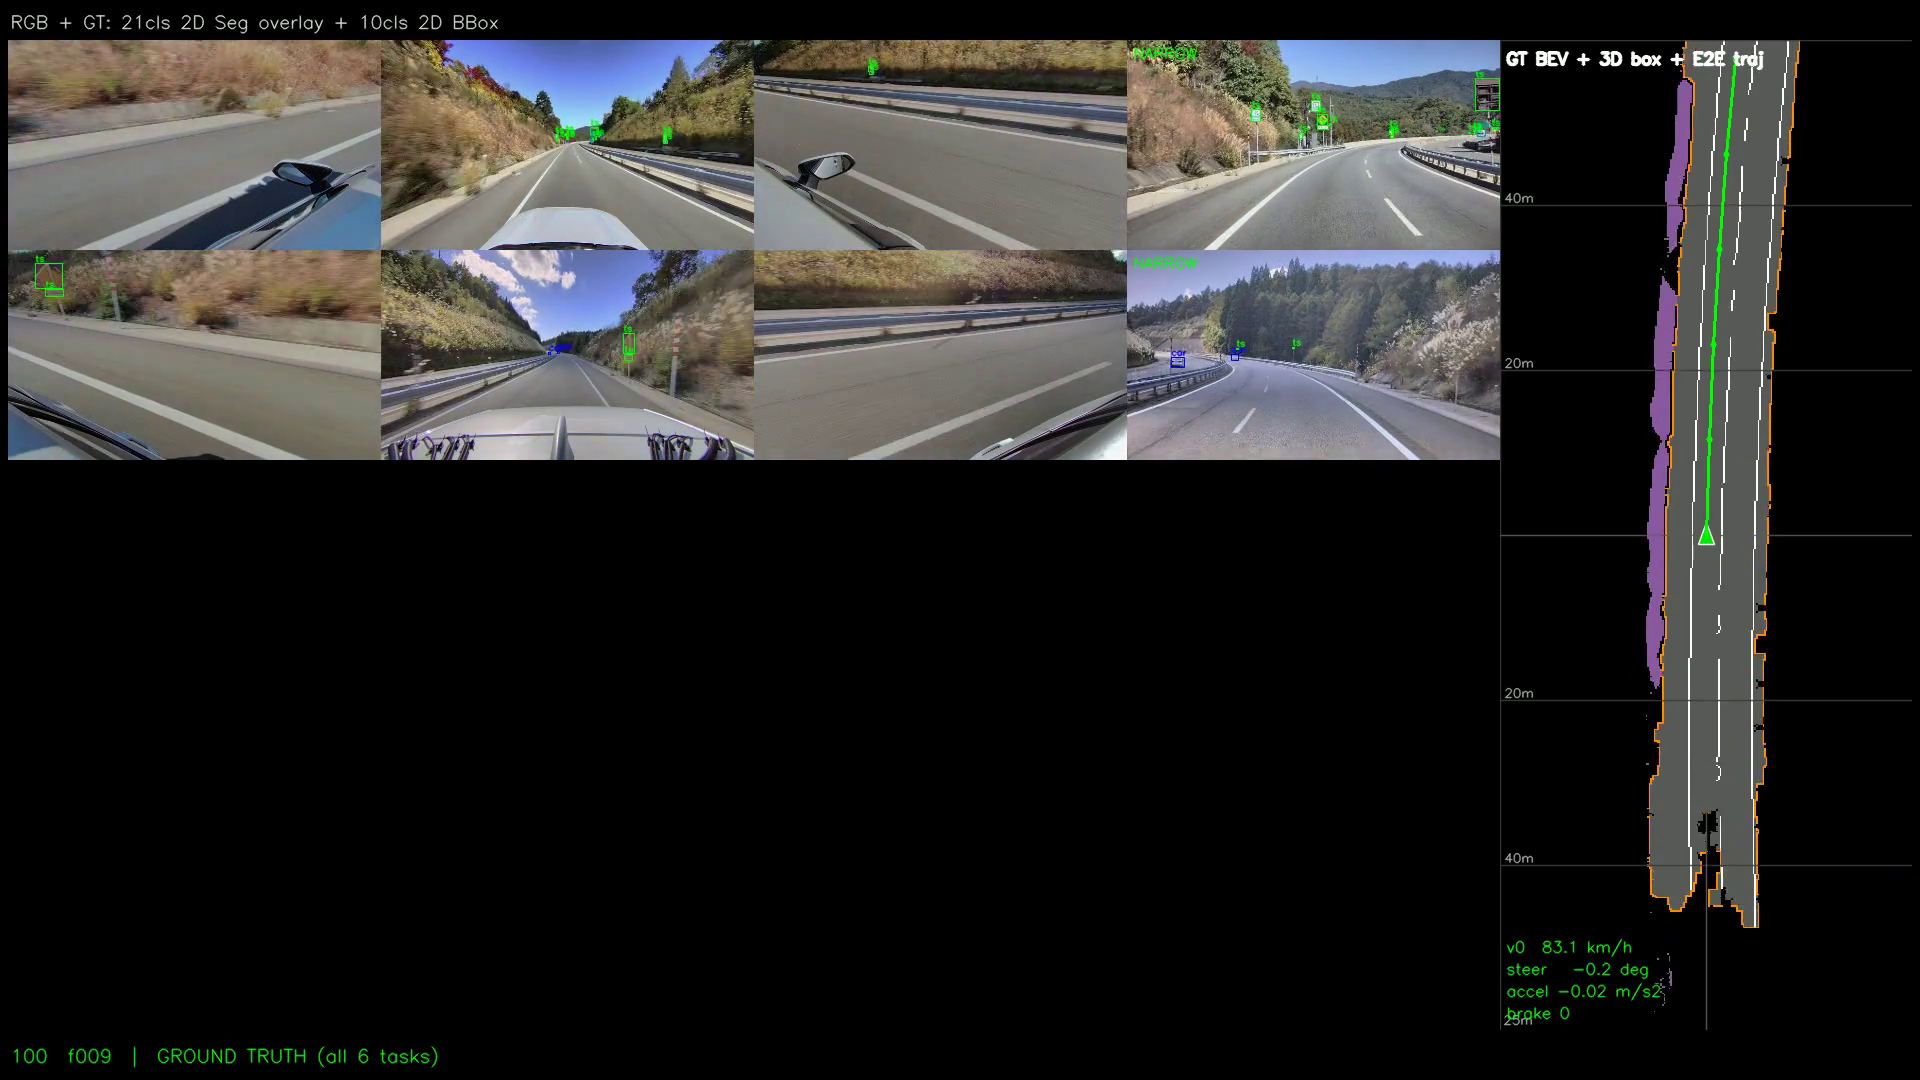
\includegraphics[width=0.99\linewidth]{figs/qual_gt.png}
\caption{\textbf{Qualitative results.} Top: single-pass inference---eight
cameras with 21-class segmentation, 2D and projected 3D boxes, and the
predicted path ribbon; metric depth; predicted occupancy (isometric); BEV
lanes with oriented boxes and the E2E trajectory with control gauges.
Bottom: the corresponding fully automatic ground truth.}
\label{fig:qual}
\end{figure}

\section{Agent-Authored Development}
\label{sec:agent}
Every artefact of this project---the ten GT extractors, twenty model
variants, the trainer, the demo renderers, the documentation, and this
manuscript---was written by a large language model agent (Claude Fable~5,
Anthropic) operating in an autonomous loop: humans supplied goals and
critiques in natural language ($\approx$70 instructions over the reported
period) and reviewed rendered videos and metrics; the agent designed,
implemented, launched and monitored training, diagnosed failures from its own
measurements, and iterated. Several of the fixes reported above originated
from the agent's own diagnostics (\eg{} the KMAX truncation analysis); others
from human observations that the agent then localised and repaired (\eg{} the
scene-tail speed bug). We do not claim the agent is autonomous in the strong
sense---direction remained human---but the division of labour (humans specify
\emph{what}, the agent implements, measures, and explains \emph{how}) held
for 100\% of the code, and we found the resulting cadence (nine training
rounds and four new task heads in three days) difficult to reconcile with
conventional development.

\section{Limitations}
Thin-class BEV IoU (lane line 0.14, stop line 0.11) remains low in absolute
terms; the labels themselves carry residual noise near intersections, and
IoU on 1-px-wide classes is a harsh metric. The E2E head is pure imitation
without commands or multi-modality, so intersections are resolved by
data prior rather than intent. Occupancy hallucination in unknown regions is
mitigated but not eliminated by denser carving; a principled treatment of
camera visibility masks~\citep{tian2023occ3d} is future work. Validation
uses a single held-out recording; broader-scale evaluation across platforms
awaits the full corpus conversion. Finally, the network is single-frame;
temporal fusion is an obvious next step.

\section{Conclusion}
\meteor{} demonstrates that a competitive seven-task surround-view driving
network can be built from raw fleet recordings with no human annotation and,
in this instance, no human-written code---the autolabel factory of the
Co-MLOps project (CoMET) supplies every supervision signal, and an LLM agent
supplied every line of implementation. We believe the combination---data
platforms that record everything, factories that label everything, agents
that implement anything specified---changes the economics of adding a task
from ``a labeling campaign'' to ``a prompt and a GPU-day,'' and we offer the
system, its measurements, and its failure catalogue as evidence.

\medskip
\noindent\textbf{Acknowledgements.} Built on the CoMET autolabeling
foundation of the Co-MLOps project. Presented at NVIDIA GTC 2026 (session
S81897).

\bibliographystyle{unsrtnat}
\begin{thebibliography}{20}\small

\bibitem{philion2020lss}
J.~Philion and S.~Fidler.
\newblock Lift, splat, shoot: Encoding images from arbitrary camera rigs by
implicitly unprojecting to 3d.
\newblock In \emph{ECCV}, 2020.

\bibitem{li2023bevdepth}
Y.~Li et~al.
\newblock BEVDepth: Acquisition of reliable depth for multi-view 3d object
detection.
\newblock In \emph{AAAI}, 2023.

\bibitem{li2022bevformer}
Z.~Li et~al.
\newblock BEVFormer: Learning bird's-eye-view representation from
multi-camera images via spatiotemporal transformers.
\newblock In \emph{ECCV}, 2022.

\bibitem{huang2023tpvformer}
Y.~Huang et~al.
\newblock Tri-perspective view for vision-based 3d semantic occupancy
prediction.
\newblock In \emph{CVPR}, 2023.

\bibitem{hu2023uniad}
Y.~Hu et~al.
\newblock Planning-oriented autonomous driving.
\newblock In \emph{CVPR}, 2023.

\bibitem{liao2023maptr}
B.~Liao et~al.
\newblock MapTR: Structured modeling and learning for online vectorized hd
map construction.
\newblock In \emph{ICLR}, 2023.

\bibitem{yin2021centerpoint}
T.~Yin, X.~Zhou, and P.~Kr\"ahenb\"uhl.
\newblock Center-based 3d object detection and tracking.
\newblock In \emph{CVPR}, 2021.

\bibitem{zhou2019objects}
X.~Zhou, D.~Wang, and P.~Kr\"ahenb\"uhl.
\newblock Objects as points.
\newblock \emph{arXiv:1904.07850}, 2019.

\bibitem{tian2023occ3d}
X.~Tian et~al.
\newblock Occ3D: A large-scale 3d occupancy prediction benchmark for
autonomous driving.
\newblock In \emph{NeurIPS}, 2023.

\bibitem{codevilla2018cil}
F.~Codevilla et~al.
\newblock End-to-end driving via conditional imitation learning.
\newblock In \emph{ICRA}, 2018.

\bibitem{qi2021offboard}
C.~R. Qi et~al.
\newblock Offboard 3d object detection from point cloud sequences.
\newblock In \emph{CVPR}, 2021.

\bibitem{caesar2020nuscenes}
H.~Caesar et~al.
\newblock nuScenes: A multimodal dataset for autonomous driving.
\newblock In \emph{CVPR}, 2020.

\bibitem{he2016resnet}
K.~He, X.~Zhang, S.~Ren, and J.~Sun.
\newblock Deep residual learning for image recognition.
\newblock In \emph{CVPR}, 2016.

\bibitem{lin2017fpn}
T.-Y. Lin et~al.
\newblock Feature pyramid networks for object detection.
\newblock In \emph{CVPR}, 2017.

\bibitem{lin2017focal}
T.-Y. Lin et~al.
\newblock Focal loss for dense object detection.
\newblock In \emph{ICCV}, 2017.

\bibitem{berman2018lovasz}
M.~Berman, A.~Rannen~Triki, and M.~B. Blaschko.
\newblock The Lov\'asz-softmax loss: A tractable surrogate for the
optimization of the intersection-over-union measure in neural networks.
\newblock In \emph{CVPR}, 2018.

\bibitem{salehi2017tversky}
S.~S.~M. Salehi, D.~Erdogmus, and A.~Gholipour.
\newblock Tversky loss function for image segmentation using 3d fully
convolutional deep networks.
\newblock In \emph{MLMI}, 2017.

\end{thebibliography}

\end{document}
